\section{Pipeline}
\label{sec:pipeline}

The pipeline described here is the last of a series. Its first version predated
any observed failure: humans handed the agent two papers, on statistical schema
profiling~\cite{metadata-extraction} and on agentic data
exploration~\cite{apex-sql}, neither with a public implementation at the time,
and the agent reproduced both from the text alone. Later versions grew inside
the loop of Section~\ref{sec:methodology}, within which the agent chose its own
reading and consulted the systems at the top of the BIRD
leaderboard~\cite{bird-leaderboard} when a failure pointed at an established
technique. The seed was not exempt from the gate: the profiling half is still
in the pipeline below, and the exploration half was scored out by a later full
run.

Seventeen steps survived, in a fixed order, in five groups
(Figure~\ref{fig:steps}): three for table selection,
five for schema building, two for generation and review, four targeted
repairs, and three normalizers. A step receives the question, its evidence
hint, and everything the earlier steps recorded, and it either extends that
context or rewrites the query.

\begin{figure*}[t]
  \centering
  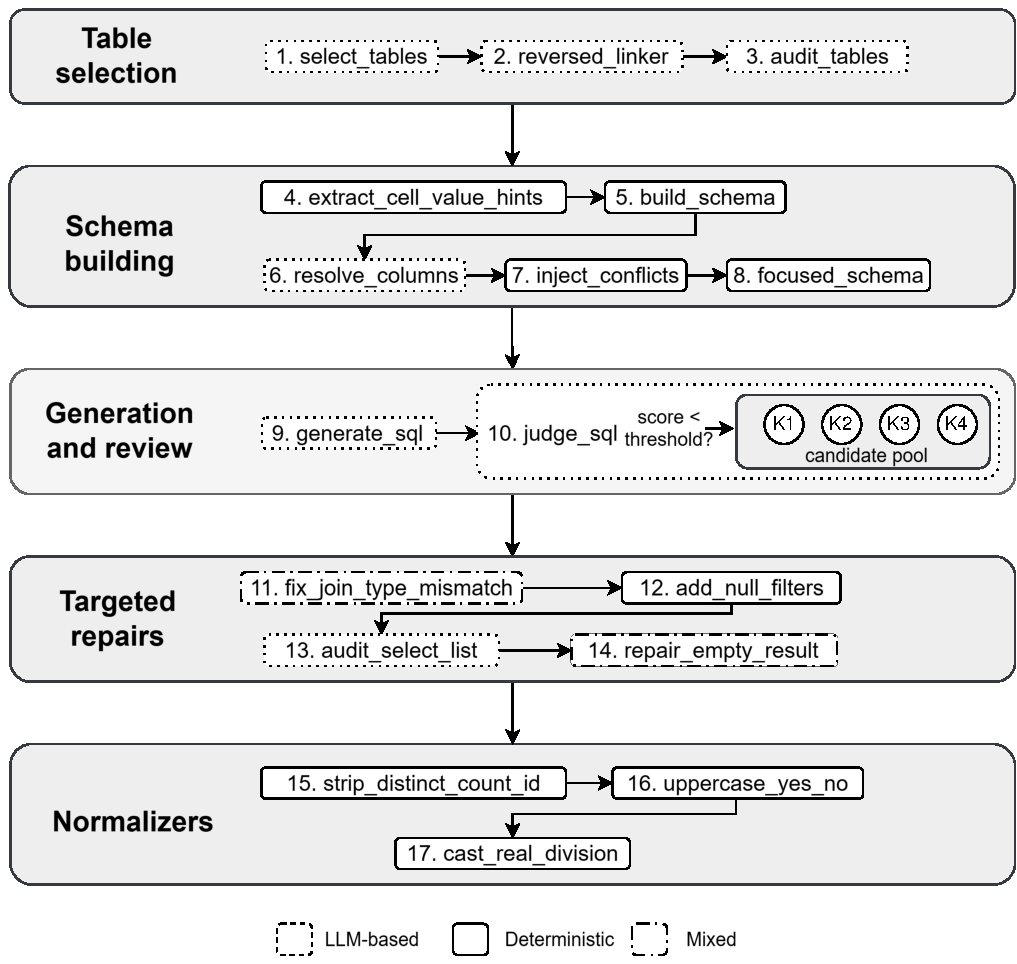
\includegraphics[width=0.78\textwidth]{steps_iccq-fig}
  \caption{The 17 steps as data flow, named by their identifiers in the
  pipeline source and grouped by function. The border style marks how a step
decides:
  by a call to a language model, by deterministic code, or by a mix in
  which deterministic code detects the defect, a language model drafts the
  rewrite, and a deterministic check accepts or discards it. Context
  accumulates until generation, and every step after it either passes the
  query through untouched or rewrites it behind its guards.}
  \label{fig:steps}
\end{figure*}

\paragraph{The shared conservative design.} What makes a chain of seventeen
rewrites viable is a shared conservative design. Each step is an opportunity to
break a query that was already correct, and the opportunities compound unless
every step passes a correct query through untouched. Four properties do that
work. Each step bounds the worst case it can produce and keeps that bound
small. Each fires only on positive evidence, so a query with no symptom leaves
a step exactly as it arrived. Detection is deterministic wherever the schema or
the syntax of the query supplies the evidence. And where a model call is
involved, it drafts the rewrite but never decides whether the rewrite is kept:
a check on the rewritten query accepts it or restores the query the step
received. The gate selected this design rather than prescribing it. An unguarded
rewrite repairs the questions it was written for and breaks others it never
considered, so its net effect over 1,534 questions comes out small or negative
and the step does not survive.

\paragraph{Table selection.} Three model calls narrow the database to the
tables a question needs. \texttt{select\_tables} proposes a set from a profile
computed once per database~\cite{metadata-extraction}: row counts, NULL rates,
numeric ranges, and value distributions, with low-cardinality columns
enumerated in full. Those statistics make the later choices value-grounded, so
a literal in the question can be matched against a column's actual domain
rather than against its name. \texttt{reversed\_linker} works
backwards~\cite{deepeye-sql}: instead of asking for a list of tables, it asks
for a draft query over the full catalog, discards the draft, and keeps the
tables the draft referenced, which recovers the bridge tables a name-matching
selector misses.
\texttt{audit\_tables} asks once whether anything relevant is still missing.
All three are recall-biased for the same reason: a missing table cannot be
recovered downstream, while an extra one costs tokens. The worst case is
bounded by monotonicity: the two steps after the selector can only add tables
to its set, and a failure inside the selector falls back to every table in
the database.

\paragraph{Schema building.} Five steps turn the selected tables into the text
the generator reads. \texttt{extract\_cell\_value\_hints} scans the question
for phrases stored verbatim as cell values and records the table and column
where each one lives~\cite{deepeye-sql}. \texttt{build\_schema} renders the
selected tables as an extended M-Schema~\cite{xiyan-sql} carrying the same
profiling statistics, and every step downstream reads the database through that
rendering. \texttt{resolve\_columns} binds each concept in the question to
exactly one column and must list the plausible alternatives it rejected as
conflicts. That binding is a contract downstream, and the run records exposed
its failure mode: a concept bound to a look-alike with an empty conflict list
freezes the error, because the generator never sees the column it should have
chosen instead. \texttt{inject\_conflicts} reopens those cases, retrieving
look-alikes by name overlap and embedding rank~\cite{qwen3-embedding} for every
concept the previous step left conflict-free. In the final run it added
conflict sets to 1,201 of the 1,534 questions, 2,227 concepts in all.
\texttt{focused\_schema} trims the rendering down to the resolved columns,
their conflicts, and every key, so the join paths survive. The trim is where
the group's worst case is bounded: it may not drop a column that either of
the two binding steps put in play, so every resolved column reaches the
generator.

\paragraph{Generation and review.} \texttt{generate\_sql} turns the question,
the evidence hint, the focused schema, the column bindings, and the cell-value
hints into a query in one call to the strongest available model. A query that
executes and returns zero rows counts as a failure and triggers one
regeneration. No reference answer on the development set is empty, so a
valid-but-empty result is always wrong. \texttt{judge\_sql} then scores the
query. At or above a threshold the pipeline spends nothing further on review.
Below it, the step assembles a pool of four candidates: the original, a
corrective rewrite of it, a variant generated with explicit reasoning, and a
variant generated from a decomposition of the question. Candidates whose result
rows are identical collapse into one, and a winner is chosen by pairwise
votes~\cite{agentar-scale-sql}, with every tie and every unparsable vote
resolving toward the original. The threshold is what makes the pool affordable.
In the final run it opened on 118 of the 1,534 questions.

\paragraph{Targeted repairs.} Four steps each own one defect signature that
kept recurring in the run records. \texttt{fix\_join\_type\_mismatch} parses
the query and compares the declared types of the columns each join equates. A
join across an INTEGER key and a TEXT key is detected from the schema alone, a
model drafts the rewrite, and the rewrite is kept only if the mismatch is gone
and rows come back. \texttt{add\_null\_filters} guards an \texttt{ORDER
BY \dots{} LIMIT} whose top row carries a NULL sort key---a shape that returns
a row answering nothing. \texttt{audit\_select\_list} is confined to the
projection, where it repairs a look-alike column, a plural question answered
with a single column, or one field too many. It may touch nothing else, and it
answered OK on 1,515 of the 1,534 questions of the final run.
\texttt{repair\_empty\_result} is the backstop for the empty-result symptom:
read-only probes establish why the result is empty, a model drafts a rewrite
from what they found, and the step discards about half of those drafts on its
own validity checks. Its position is load-bearing. It runs last among the steps
that can change which rows come back, because an earlier arrangement let
\texttt{audit\_select\_list} run afterwards and revert a repaired query to
empty. Two of these four did not fire once across the final run, their
signatures squeezed out upstream as selection and generation improved. Both
stay, since detection is deterministic and an idle pass costs nothing.

\paragraph{Normalizers.} Three deterministic passes over the parsed query close
the pipeline, and none changes which rows the query returns.
\texttt{strip\_distinct\_count\_id} removes \texttt{DISTINCT} from counts over
identifier columns, \texttt{uppercase\_yes\_no} raises lowercase yes and no
literals to the casing the reference answers use, and
\texttt{cast\_real\_division} inserts a cast where a projection divides one
integer by another. Every join and every filter passes through untouched, which
is what licenses running these three after the backstop. What they rewrite is
how the answer is expressed: whether a count deduplicates, how a literal is
cased, whether a division truncates. When results are compared as sets of
rows, those details alone separate a right answer from a wrong one, so a
rewrite there can flip a verdict in either direction.

\paragraph{One step in detail.} \texttt{strip\_distinct\_count\_id} shows what
the guards are worth. Asked how many X there are, the model defensively writes
\texttt{COUNT(DISTINCT id)} where the reference query counts joined rows as
they come, and the two answers diverge exactly when a join fans out. Three of
the step's four guards are simple: the question must not itself ask for
distinctness, every counted column must be identifier-shaped, and the stripped
query must still execute. The fourth is a confidence gate on the judge's score,
calibrated by replaying the strip against the recorded results of all 1,534
development questions and sweeping the cutoff, which shows for every candidate
value which questions it repairs and which it breaks. The chosen value sits in
the middle of the band the sweep marked safe, away from the edge where the
strip starts breaking correct answers. In the final run 89 queries reached the
step carrying a \texttt{COUNT(DISTINCT \dots{})} and 51 were rewritten, the
step standing down on 21 whose question asked for distinctness, 8 counting a
column that was not identifier-shaped, and 9 the judge had endorsed above the
gate.

Read against RQ2, every step after generation descends from a defect signature
the run records made legible and some check could then recognize. A query that
executes to zero rows, on a benchmark where no reference answer is empty,
licenses \texttt{repair\_empty\_result}. A concept bound to a look-alike with
no alternative recorded licenses \texttt{inject\_conflicts}. A defensive
\texttt{COUNT(DISTINCT \dots{})} over an identifier column licenses
\texttt{strip\_distinct\_count\_id}. A join equating columns of different
declared type licenses \texttt{fix\_join\_type\_mismatch}. Every pair is the
same move: a defect visible in the records became a predicate, and the
predicate became the guard on a rewrite. Defects the records exposed but no
predicate could recognize produced no step at all.
